%% SECTION HEADER /////////////////////////////////////////////////////////////////////////////////////
\section{Piezoelectric Transducers}
\label{sec:PZT}

%% SECTION CONTENT ////////////////////////////////////////////////////////////////////////////////////
The piezoelectric phenomenon is the generation of an electrical charge on the surface of materials under mechanical deformation in crystalline materials with no inversion symmetry.
The magnitude of the generated charge is proportional to the strain and the direction of polarization.
Those materials also exhibit the opposite effect: a change in size due to an applied electric field.
Piezoelectric materials are widely used in engineering as electroacoustic transducers, high voltage generators and power sources, energy harvesters, micro motors and actuators.
\begin{figure}[H]
	%	\begin{center}
	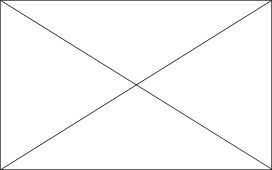
\includegraphics[width=1\linewidth]{Intro/placeholder}
	%	\end{center}
	\caption{Various types of piezoelectric transducers.}
	\label{fig:piezo}
\end{figure}
\Acp{pzt}, the acronym derived from the chemical formula of the most commonly used piezoelectric ceramic, i.e. Pb[Zr\(_x\)Ti\(_{1-x}\)]O\(_3\) (lead zirconate titanate), are lightweight, various size and shape structures. 
They can be permanently mounted on the structure surface, embedded within the material, or even be a smart composite material.
In \ac{shm}, they are mainly used in elastic wave propagation, modal analysis, and \ac{emi} methods.